\chapter{Resultados e discussão}\label{cap:resultados}
Esta seção apresenta os resultados dos testes e registros produzidos pelos autores durante o desenvolvimento do DoseCerta. A análise diferencia configurações, versões, testes automatizados, respostas dos controladores e observações físicas. Os resultados exploratórios não são apresentados como validação clínica nem como campanha controlada da configuração final.

O módulo HW-084 com DS3231M estava presente, mas, em 26 de novembro, não estava ativado no Linux; a referência temporal confiável dependia da rede. A bateria compatível ainda precisava ser conferida.

\section{Configuração registrada}
Às 22h10 de 26 de novembro, a central registrava runtime 0.9.2, release \texttt{2026.11.25-cam-3}, INT01 0.3.1 e SUB01 0.6.1, em ambiente Simulado. O provisionamento documentado é 0.1.0+dc9. As duas placas respondiam na coleta posterior, superando o relato de indisponibilidade de 25 de novembro, mas sem demonstrar a correção da causa. O RTC não estava habilitado no Linux e a dispensação agendada permanecia desligada. As fotografias da Seção~\ref{cap:mecanica} documentam a montagem, e a Tabela~\ref{tab:v75-dimensoes} apresenta as cotas nominais V75. A inspeção dimensional das peças impressas permanece uma avaliação distinta. 
\pendencia{RES01}{Acrescentar os resumos criptográficos e o manifesto sanitizado da configuração que será apresentada, instrumentos e condição de comissionamento. A configuração lida em 26/11 não reúne todos os ensaios históricos desta seção.}

\section{Mecânica, calibração e elétrica}
As três calibrações salvas têm 15 intervalos, média de 819,2 fases, desvio-padrão amostral de aproximadamente 11,2, mínimo 806 e máximo 846. Cada perfil fecha 4.096 fases por construção da representação; a média coincide com $4.096/5$ e não comprova precisão angular absoluta. Não há encoder nem conferência independente de repetibilidade angular. 

O perfil ativo de 7 de novembro, 23h24, apresenta centros em 0, 814, 1.639, 2.451 e 3.266 fases e intervalos 814, 825, 812, 815 e 830. A faixa de vazio é 1.556--2.920 e a de ocupado 1--1.139. A separação de 417 contagens entre as faixas do perfil ativo não é taxa de classificação: a maior leitura ocupada entre os três perfis é 1.148, portanto a síntese ``ocupado até 1.139 nas três calibrações'' seria imprecisa. 

A influência óptica do reservatório e a intervenção com fita preta são analisadas adiante nesta seção. Não foram realizadas medições dimensionais da peça fabricada, corrente em atuação ou tensão transitória no SUB01. A queda de alimentação é diagnóstico confirmado em uma ocorrência de brownout; não foi demonstrada como causa única de todos os reinícios. 
\pendencia{RES02}{Comparar cotas físicas com as dimensões nominais V75 já incorporadas; completar corrente e tensão sob carga, aquecimento e ensaios pós-reparo. Inclinação nominal final definida em 30° em relação à vertical.}

As faixas salvas são comparadas na Figura~\ref{fig:result-faixas}; representam perfis, não uma distribuição de erros de classificação.

\begin{figure}[H]
\centering
\caption{Faixas ADC de ocupado e vazio nos três perfis salvos}\label{fig:result-faixas}
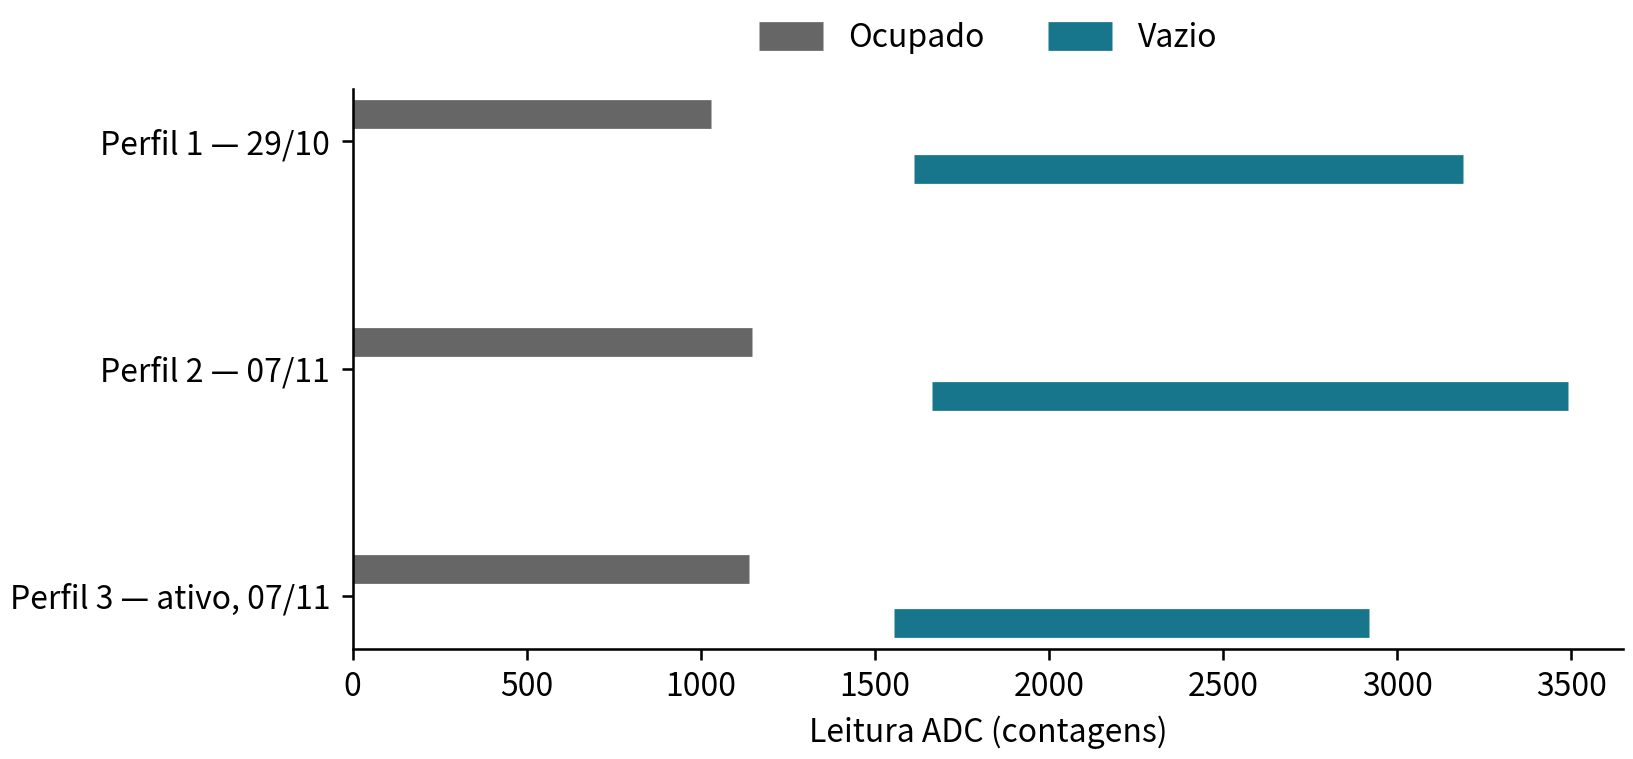
\includegraphics[width=0.94\textwidth,keepaspectratio]{Figuras/Validacao20261126/faixas_calibracao.png}
\fonte{Autoria própria (2026).}
\end{figure}

\noindent

\section{Comunicação e controle embarcado}
O registro DC1 contém 3.430 comandos entre 17 de outubro e 26 de novembro, em 17 dias de uso: 2.669 para INT01 e 761 para SUB01. Os identificadores registrados são únicos e contíguos por placa. Isso caracteriza o banco examinado; não prova ausência de toda tentativa de transmissão ou duplicação física não registrada. Das entradas, 3.071 estão em \texttt{ACKNOWLEDGED} e 359 em \path{MOTION_ACKNOWLEDGED}. Estados capturados como \texttt{BUSY} não equivalem a movimentos concluídos. 

Há 39 comandos ABORT com resposta de parada e 303 giros \texttt{BENCH\_JOG} concluídos, somando 139.244 fases. São respostas do firmware, não 39 medições independentes de tempo físico de parada nem 303 dispensações contadas. A telemetria posterior distingue leituras de estado das operações de motor. 

{\small\setlength{\tabcolsep}{3pt}
\begin{longtable}{p{0.35\textwidth}p{0.17\textwidth}p{0.17\textwidth}p{0.17\textwidth}}
\caption{Localização e calibração por fase do software}\label{tab:result-sessoes}\\
\hline\textbf{Ação} & \textbf{Até dc8-3} & \textbf{dc8-4/5} & \textbf{dc8-6 em diante}\\\hline\endfirsthead
\hline\textbf{Ação} & \textbf{Até dc8-3} & \textbf{dc8-4/5} & \textbf{dc8-6 em diante}\\\hline\endhead
Localização concluída / sessões & 1/12 & 3/7 & 2/2\\\hline
Calibração \texttt{calibrate\_slot} concluída / sessões & 1/18 & 2/5 & 0/3\\\hline
\end{longtable}
\noindent Fonte: Autoria própria (2026).\par}
A operação distinta \texttt{calibrate\_five} tem uma sessão concluída e não foi somada à linha de \texttt{calibrate\_slot}. O resultado 2/2 de localização pertence ao grupo histórico dc8-6 em diante; não é amostra específica da release 0.9.2 nem comprova a meta proposta de 98\%.

\subsection{Dispensação: sessão, ciclo e quantidade física}
As 15 sessões \texttt{simulate\_quantity} totalizam 21 unidades solicitadas. Doze sessões têm estado de software concluído, mas apenas quatro possuem motivo final \path{slot_quantity_completed}; outras foram encerradas por retenção ou impedimento de prosseguir. Os 12 ciclos com registro por cavidade são classificados na Tabela~\ref{tab:result-ciclos}. Nenhuma dessas grandezas fornece, por si, a quantidade contada no copo. 

{\small\begin{longtable}{p{0.64\textwidth}p{0.23\textwidth}}
\caption{Desfechos registrados dos 12 ciclos de dispensação}\label{tab:result-ciclos}\\
\hline\textbf{Classificação do registro} & \textbf{Ciclos}\\\hline\endfirsthead
\hline\textbf{Classificação do registro} & \textbf{Ciclos}\\\hline\endhead
Cavidade verificada vazia após retorno & 4\\\hline
Saída com reabastecimento, segundo o controlador & 2\\\hline
Unidade retida & 4\\\hline
Intenção de ciclo sem releitura & 2\\\hline
\end{longtable}\noindent Fonte: Autoria própria (2026).\par}

Quatro dos dez ciclos com releitura foram classificados como retenção. Essa proporção descreve a pequena amostra disponível, não a taxa de erro final do produto. Os dois casos de reabastecimento terminam com leitura ocupada ou ambígua, de modo que a interpretação do controlador precisa permanecer separada da observação física. Sem contagem humana por ciclo, não se calcula taxa pedido = saída nem se demonstra ausência de dose dupla. 
\pendencia{RES03}{Executar a campanha com contagem independente, referência física, versões e denominadores: acerto, ausência, unidade extra, retenção, travamento, tempo e recuperação. Preservar tentativas interrompidas.}

A Figura~\ref{fig:result-ciclos} sintetiza as categorias de registro, sem equipará-las à saída observada no coletor.

\begin{figure}[H]
\centering
\caption{Categorias dos ciclos registrados, sem contagem física independente}\label{fig:result-ciclos}
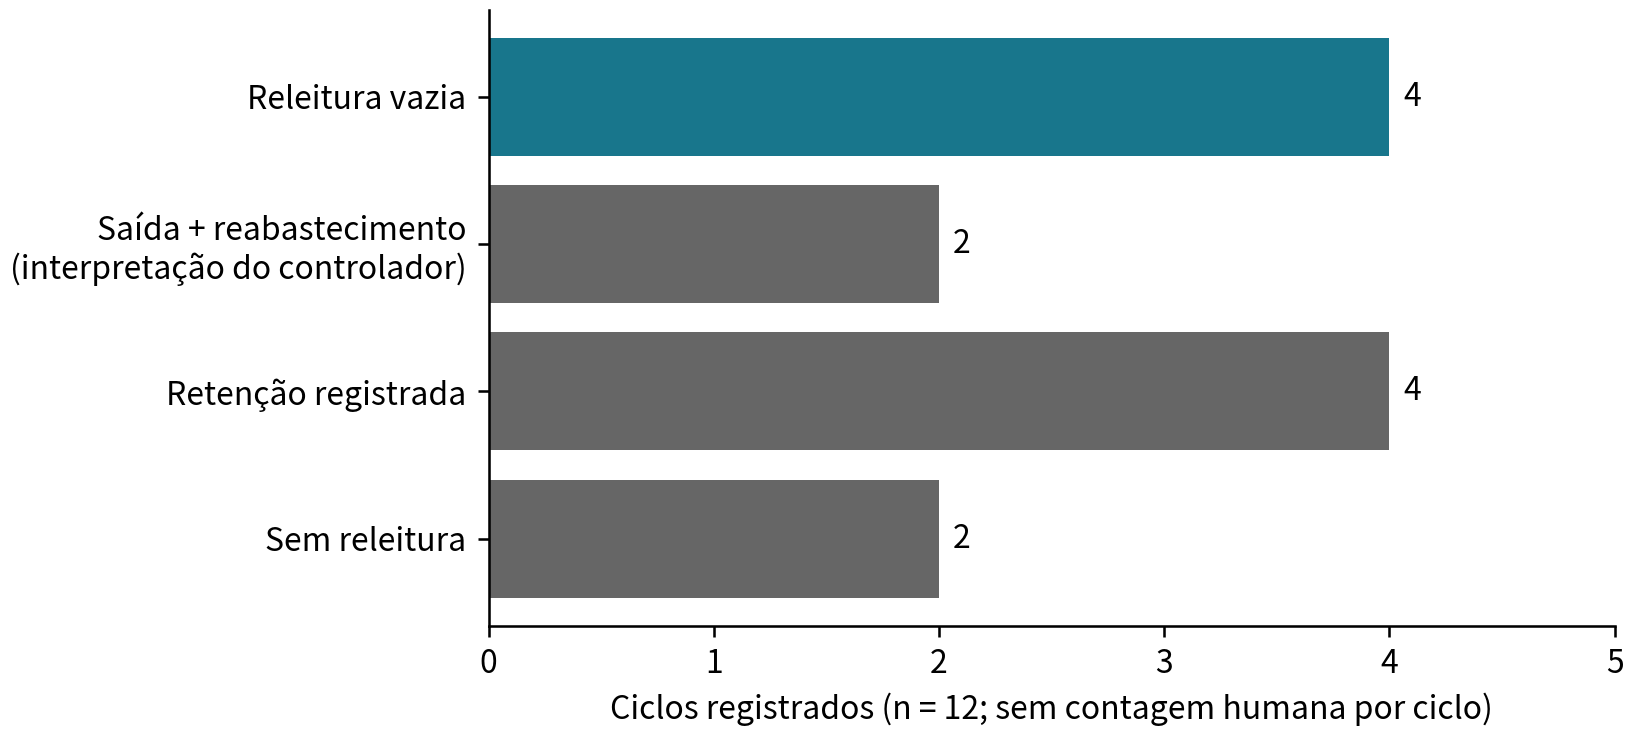
\includegraphics[width=0.94\textwidth,keepaspectratio]{Figuras/Validacao20261126/desfechos_ciclos.png}
\fonte{Autoria própria (2026).}
\end{figure}

\noindent

\section{Resultados da dispensação vinculada}
Foram analisados, no Oficial, oito registros iniciados entre 29 de outubro e 8 de novembro, não oito execuções homogêneas bem-sucedidas. Três pedidos (2, 6 e 7) foram recusados antes de mover e têm relato de zero saída. Há três ciclos completos com veredito: no 3, o sensor indica retenção e o relato é zero; no 4, leitura vazia e relato de uma unidade; no 5, retenção e resposta ``não observado''. O 8 requer reconciliação, com relato de uma unidade. O 1 recebe relato de saída cerca de nove dias depois do pedido, apesar de zero ciclos associados; permanece identificado como inconsistente. 

% Gerado em 26/11/2026 a partir do banco de produção (eventos bound_dispense e comandos dc1_motor).
% Só ensaios do ambiente Oficial (política "rigoroso"), 29/10 a 08/11/2026. Desde 14/11 o aparelho está no
% ambiente Simulado (banco tcc_simulado, política "apresentacao"); esses ensaios estão em ensaios_dispensacao_simulado.csv.
% Estilo igual às longtables da monografia (Capitulos/05_requisitos.tex).

{\small\setlength{\tabcolsep}{3pt}\begin{longtable}{p{0.035\textwidth}p{0.105\textwidth}p{0.04\textwidth}p{0.05\textwidth}p{0.155\textwidth}p{0.18\textwidth}p{0.13\textwidth}p{0.105\textwidth}}
\caption{Ensaios de dispensação integrada no submódulo SUB01 (aplicativo, API, central e ESP32)}\label{tab:ensaios-dispensacao}\\
\hline
\textbf{N.} & \textbf{Início} & \textbf{Qtd.} & \textbf{Ciclos} & \textbf{Sensor antes/depois} & \textbf{Resultado do aparelho} & \textbf{Observação humana} & \textbf{Estoque}\\\hline
\endfirsthead\hline
\textbf{N.} & \textbf{Início} & \textbf{Qtd.} & \textbf{Ciclos} & \textbf{Sensor antes/depois} & \textbf{Resultado do aparelho} & \textbf{Observação humana} & \textbf{Estoque}\\\hline
\endhead
1 & 29/10 13h34 & 1 & 0 & -- & Falha antes do ciclo (leitura do ADC alterada) & Saída de 1 (registrada em 07/11) & 13 $\rightarrow$ 12\\\hline
2 & 07/11 23h25 & 2 & 0 & -- & Recusa: estado inicial ambíguo & Sem saída & 12 $\rightarrow$ 12\\\hline
3 & 08/11 09h37 & 1 & 1 & 154 ocupado / 223 ocupado & Unidade retida & Sem saída & 12 $\rightarrow$ 12\\\hline
4 & 08/11 13h26 & 1 & 1 & 108,5 ocupado / 1916,5 vazio & Saída concluída & Saída de 1 & 12 $\rightarrow$ 11\\\hline
5 & 08/11 13h27 & 2 & 1 & 139 ocupado / 144 ocupado & Unidade retida (2 tentativas de desobstrução) & Não observado & 11 / pós ausente\\\hline
6 & 08/11 21h32 & 1 & 0 & -- & Recusa: estado inicial ambíguo & Sem saída & 11 $\rightarrow$ 11\\\hline
7 & 08/11 21h32 & 1 & 0 & -- & Recusa: estado inicial ambíguo & Sem saída & 11 $\rightarrow$ 11\\\hline
8 & 08/11 21h38 & 1 & 1 & 388 ocupado / -- & Ciclo interrompido; exige reconciliação & Saída de 1 & 11 $\rightarrow$ 10\\\hline
\end{longtable}}{\small\noindent Fonte: Autoria própria (2026).\par}


{\small\setlength{\tabcolsep}{3pt}\begin{longtable}{p{0.65\textwidth}p{0.25\textwidth}}
\caption{Qualidade e elegibilidade dos oito registros do Oficial}\label{tab:indicadores-dispensacao}\\
\hline\textbf{Critério de leitura} & \textbf{Registros}\\\hline\endfirsthead
\hline\textbf{Critério de leitura} & \textbf{Registros}\\\hline\endhead
Total de linhas no CSV & 8\\\hline
Quantidade observada preenchida & 7/8\\\hline
Observação tardia incompatível com o ciclo & 1 (ensaio 1)\\\hline
Sem quantidade observada e sem estoque posterior & 1 (ensaio 5)\\\hline
Linhas com quantidade e estoque antes/depois, excluído o caso tardio & 6 (2, 3, 4, 6, 7 e 8)\\\hline
Nessas seis, redução do estoque registrado igual à quantidade relatada & 6/6; consistência contábil\\\hline
Saídas unitárias relatadas sem a inconsistência temporal do ensaio 1 & 2 (4 e 8)\\\hline
Recusas antes de mover com relato de zero saída & 3 (2, 6 e 7)\\\hline
Ciclo retido com relato de zero saída & 1 (3)\\\hline
\end{longtable}\noindent Fonte: Autoria própria (2026).\par}


Não se adota a síntese ``estoque correto em 8/8'': a linha 5 não tem estoque posterior nem quantidade observada, e a linha 1 não serve como correspondência temporal confiável. Nas seis linhas restantes, a redução registrada corresponde à quantidade relatada, mas isso comprova apenas consistência contábil dos registros. Não há contagem física independente do reservatório que demonstre integridade em todas as linhas. Da mesma forma, a ausência de unidade extra nos relatos completos não é garantia de ausência de dose dupla nos oito casos. Não se calcularam estimativas de eficácia ou segurança a partir de registros com observação incompleta. 

A Tabela~\ref{tab:ensaios-simulado} contém sete linhas de 14 de novembro. O campo \texttt{fechamento} registra quatro encerramentos automáticos, dois relatos humanos de demonstração e uma linha sem fechamento. Portanto, cinco casos estão sem quantidade humana, mas apenas quatro estão explicitamente encerrados automaticamente. Nos dois relatos de demonstração, foram informadas duas unidades, com retenção indicada pelo sensor e estoque registrado 10 para 10. Não se mistura essa política com as travas do Oficial. 

% Ensaios no ambiente Simulado (banco tcc_simulado, política "apresentacao"), 14/11/2026.
{\small\setlength{\tabcolsep}{3pt}\begin{longtable}{p{0.04\textwidth}p{0.09\textwidth}p{0.05\textwidth}p{0.19\textwidth}p{0.21\textwidth}p{0.24\textwidth}}
\caption{Ensaios de dispensação no ambiente simulado (política de apresentação)}\label{tab:ensaios-simulado}\\
\hline
\textbf{N.} & \textbf{Início} & \textbf{Qtd.} & \textbf{Sensor antes/depois} & \textbf{Resultado do aparelho} & \textbf{Fechamento}\\\hline
\endfirsthead\hline
\textbf{N.} & \textbf{Início} & \textbf{Qtd.} & \textbf{Sensor antes/depois} & \textbf{Resultado do aparelho} & \textbf{Fechamento}\\\hline
\endhead
1 & 14/11 17h02 & 1 & 122 ocupado / -- & Falha: leitura do ADC alterada & Automático, sem contagem\\\hline
2 & 14/11 18h15 & 1 & 147 ocupado / 1872 vazio & Saída concluída & Automático, sem contagem\\\hline
3 & 14/11 18h17 & 2 & 161 ocupado / 1807 vazio & Uma cavidade disponível & Automático, sem contagem\\\hline
4 & 14/11 18h20 & 1 & 272 ocupado / 1646 vazio & Saída concluída & Automático, sem contagem\\\hline
5 & 14/11 20h51 & 2 & 220,5 ocupado / 923 ocupado & Unidade retida & Humano: saída de 2 (demonstração)\\\hline
6 & 14/11 20h52 & 2 & 125,5 ocupado / 445 ocupado & Unidade retida & Humano: saída de 2 (demonstração)\\\hline
7 & 14/11 23h04 & 2 & 154 ocupado / 880 ocupado & Concluído com recarga (2 ciclos) & Sem fechamento\\\hline
\end{longtable}}{\small\noindent Fonte: CSV do Simulado na entrega de 27 nov. 2026. \cite{DC_NICOLAS2026}\par}


Esses registros não se somam às 15 sessões nem aos 12 ciclos anteriores, pois representam parte do mesmo histórico de desenvolvimento. Eles permitem relacionar operação e observação humana sem constituir uma campanha independente. Os intervalos de ADC das capturas históricas (vazio 2.755--2.952; ocupado 104--157), registrados durante os ensaios, também não substituem as faixas do perfil ativo nem incorporam as leituras intermediárias de todos os ciclos. 

\subsection{Contagens e critérios que permanecem divergentes}
As seleções históricas de localização produziram recortes de 4/9 e, na análise por fase, 1/12, 3/7 e 2/2; sem filtro e conjunto de identificadores equivalentes, essas proporções não foram intercambiadas. O resumo 3/26 de calibração refere-se à operação \texttt{calibrate\_slot}; a sessão distinta \texttt{calibrate\_five} continua separada. Indicadores de disponibilidade derivados de número de sinais por dia (91--94\% nos ensaios históricos) não são a mesma métrica que a estimativa por lacunas de 98,90\% do levantamento histórico. Nenhum deles mede acurácia física. 

\section{Telemetria passiva da central}
A janela das 22h11 às 22h40 contém 1.725 tentativas de consulta e uma falha HTTP do runtime, restando 1.724 amostras válidas por placa. As 1.614 leituras distintas por placa totalizam 3.228 sem indicação de erro ou troca de boot nas amostras válidas. A latência da consulta local foi mediana 183,4 ms, percentil 95 de 277,7 ms e máximo de 7.932,1 ms; não se trata da latência de uma dose ou de um comando remoto. 

O ADC parado teve média 143,4, desvio-padrão 1,21 e extremos 138--148 em 1.724 amostras. A temperatura da Raspberry, em 173 leituras, variou de 53,692 a 57,458 graus Celsius, média 56,0; o indicador \texttt{throttled} foi zero nessas leituras. Há 121 amostras com fila não vazia no resumo, portanto não se afirma que todas as filas estiveram vazias durante a janela. A coleta sem movimento não avalia ruído e alimentação durante atuação. 

\section{Servidor, enlace e atualização}
No Simulado, foram registrados 98.722 relatórios de estado no intervalo de 14 a 26 de novembro, mediana entre relatórios de 10,53 s e 29 lacunas maiores que 60 s. A disponibilidade estimada do enlace é 98,90\% em 293,60 h, com 3,22 h de lacunas. Inclui desligamentos deliberados e não mede a proporção de eventos corretamente sincronizados; não pode ser comparada diretamente à meta de 99\% de sincronização. 

No Oficial, os 40 comandos de LED foram aplicados, com mediana de 1,26 s até reconhecimento. Esse recorte não caracteriza a latência do motor. O histórico de instalação contém 46 releases da Raspberry; o histórico identifica 27 instalações pelo atualizador desde 24 de outubro, três recusas antes da troca e uma reversão automática. Para ESP32 há quatro atualizações aceitas e três tentativas iniciais canceladas mantendo a imagem anterior. Não se generaliza esse histórico para toda corrupção ou interrupção possível. 

\subsection{Rodadas e limites da validação de integração}
Nos testes de 19 de outubro, foram verificados retornos de sensores, LEDs, câmera, calibração e atualização das placas; também foi observado problema físico em uma conexão magnética/pogo. Os casos exploratórios orientaram correções, mas não caracterizam uma campanha de repetibilidade do encaixe.

Em 25 de novembro foram executadas verificações de tipos, contratos entre camadas e testes de caixa preta e branca; parte das falhas dependia de hardware ou de contexto de execução. Como o registro não fornece uma nova contagem consolidada por suíte, ele complementa a análise qualitativa e não substitui os números da Tabela~\ref{tab:result-software}. A nova execução de 27 de novembro do executor da campanha não equivale à execução dos seus ensaios físicos.

\subsection{Suítes automatizadas}
A Tabela~\ref{tab:result-software} reproduz rodadas identificadas na tabela histórica, sem somá-las. Suíte completa, grupo focado, teste de navegador e interação humana são unidades diferentes.
{\small\setlength{\tabcolsep}{3pt}\begin{longtable}{p{0.28\textwidth}p{0.13\textwidth}p{0.11\textwidth}p{0.11\textwidth}p{0.11\textwidth}p{0.11\textwidth}}
\caption{Rodadas de software e seus desfechos}\label{tab:result-software}\\
\hline\textbf{Suíte / data} & \textbf{Casos} & \textbf{Aprov.} & \textbf{Falhas} & \textbf{Erros} & \textbf{Ignor.}\\\hline\endfirsthead
\hline\textbf{Suíte / data} & \textbf{Casos} & \textbf{Aprov.} & \textbf{Falhas} & \textbf{Erros} & \textbf{Ignor.}\\\hline\endhead
Runtime 0.7.7, 03/11 & 712 & 711 & 0 & 1 & 0\\\hline
Runtime 0.9.2, 25/11 & 824 & 823 & 0 & 1 & 0\\\hline
API, 25/11 & 297 & 295 & 0 & 2 & 0\\\hline
Provisionamento dc8, 03/11 & 227 & 227 & 0 & 0 & 0\\\hline
Care, 07/11 & 293 & 279 & 14 & 0 & 0\\\hline
App com isolamento, 25/11 & 363 & 347 & 12 & 0 & 4\\\hline
Executor da campanha, 26/11 & 42 & 42 & 0 & 0 & 0\\\hline
\end{longtable}\noindent Fonte: Autoria própria (2026).\par}

O erro do runtime pertence ao teste legado \texttt{test\_can\_hardware}; a API registra dois erros antigos de ambiente. O app de 25 de novembro apresenta 12 falhas e quatro ignorados mesmo na execução isolada; ``nenhuma falha nova'' não significa aprovação integral. A rodada de provisionamento corresponde a dc8 e não foi atribuída à versão dc9. 
\pendencia{RES04}{Vincular versões e logs completos do servidor e aplicativo apresentados na defesa; resolver ou justificar erros e falhas remanescentes. Completar testes autenticados de ponta a ponta e tarefas, sem somar rodadas.}

Em 18 de novembro, foram registrados 224/240 casos aprovados na suíte geral e 341/359 no Care, incluindo quatro ignorados. Não se trata de reexecução posterior à rodada de 25 de novembro; por isso, esses valores são históricos e não substituem a tabela de rodadas acima. As capturas demonstram a interface, não a aprovação dos testes ou o isolamento do paciente. 

\section{Visão, agente e avaliação de uso}
Para a implementação vision-v3, foram definidos método, parâmetros e limites, mas ainda não há conjunto de avaliação independente para cálculo de métricas. Os cinco eventos históricos originados pelo dispositivo e o evento manual de demonstração não compõem um conjunto de referência independente. Os resultados das versões anteriores são mantidos separados dos parâmetros da vision-v3. 

O desenvolvimento do agente alcançou registros até v28. Ensaios exploratórios indicaram aproximadamente 11 s até a primeira palavra em uma consulta por voz e cerca de 15 s na leitura de uma receita fictícia com quatro medicamentos. São observações pontuais, não uma distribuição de latências nem estimativa de precisão. Na versão 24, foi relatada escrita sem confirmação; o caso precisa ser relacionado ao diálogo e à configuração para comprovar o comportamento e sua eventual correção. A identidade fixa no MCP corresponde ao escopo deliberado de paciente único, não a uma seleção multipaciente implementada.

Não há ainda uma campanha sistemática com casos, repetições, referência humana e conferência dos efeitos persistidos para estimar desempenho do modelo. Testes do servidor MCP não substituem essa avaliação.
\subsection{Evolução dos testes de visão}
Em testes exploratórios de 28 de outubro, com webcam e uma pessoa, três de quatro sequências simuladas da versão 2 receberam escore entre 0,946 e 0,992; uma, com 0,884, ficou inconclusiva. Em outra rodada, seis sessões receberam rótulo positivo, incluindo mão apoiada na bochecha com cabeça inclinada, identificada como falso positivo. Um gesto de espreguiçar também levou a resposta positiva e motivou revisão das regras.

Esses achados descrevem ajuste durante o desenvolvimento, não avaliação independente da vision-v3. Os escores da regressão logística, sua janela e seus limiares não foram usados como precisão da máquina de estados final. Para essa versão permanecem necessárias sequências rotuladas e medições no aparelho.

\pendencia{RES05}{Completar os resultados de visão e agente separadamente, com método/versionamento reconciliados, conjunto de referência, falhas e denominadores.}
\pendencia{RES06}{Inserir avaliação de usabilidade e acessibilidade, caso realizada: protocolo, autorizações aplicáveis, participantes, tarefas e achados. Não há base para afirmar melhoria de adesão ou eficácia clínica.}

\section{Interferência óptica do reservatório e posição do disco}
As leituras escuras observadas com o reservatório deixaram de ser apenas uma causa desconhecida: o registro de bancada relaciona a mudança à reflexão infravermelha da sua base. No mesmo furo vazio, foram documentadas aproximadamente 1.970 contagens sem reservatório, 61 a 64 com ele e 1.617 a 1.625 após a aplicação de fita preta sob a base. A calibração com reservatório e fita foi então concluída. Trata-se de uma correção observada numa configuração, não de uma demonstração de estabilidade para diferentes materiais, iluminação ou envelhecimento. 

\section{Leituras posteriores e limites do diagnóstico elétrico}
Em novembro houve nova perda de comunicação do submódulo durante movimento após os reparos de fiação. O motivo de reinício dessa ocorrência não foi recuperado antes do reencaixe; não se pode atribuí-la conclusivamente ao mesmo brownout do primeiro registro. A recomendação de medir os 5 V junto ao SUB01 durante o giro e avaliar desacoplamento de 470~$\mu$F e 100~nF permanece uma ação de diagnóstico, não uma correção cuja montagem e eficácia estejam demonstradas. 

Na coleta de 26 de novembro, INT01 e SUB01 voltaram a responder e a telemetria sem motor não mostrou mudança de boot nas amostras válidas. A central ficou entre 53,69~°C e 57,46~°C; as leituras do indicador \texttt{get\_throttled} foram zero. Esses dados descrevem a condição monitorada da Raspberry, não a temperatura de todos os componentes nem a tensão transitória nos contatos. Não substituem ensaio elétrico com carga. 


\section{Volume e evolução dos dados}
A Tabela~\ref{tab:dados-volume} apresenta os volumes dos bancos em cada data de observação. As contagens de 26 de novembro provêm das estatísticas do PostgreSQL e são estimativas, não contagens exatas com \texttt{COUNT(*)}; não devem ser equiparadas às 98.722 linhas efetivamente extraídas no outro recorte. A maior parte corresponde aos sinais de vida da central, enviados a cada 10~s aproximadamente, e às respectivas chaves de idempotência.

{\small\setlength{\tabcolsep}{3pt}\begin{longtable}{p{0.34\textwidth}p{0.17\textwidth}p{0.17\textwidth}p{0.2\textwidth}}
\caption{Volume de registros nos bancos do servidor}\label{tab:dados-volume}\\
\hline\textbf{Tabela} & \textbf{Oficial, 12/11} & \textbf{Oficial, 26/11} & \textbf{Simulado, 26/11}\\\hline\endfirsthead
\hline\textbf{Tabela} & \textbf{Oficial, 12/11} & \textbf{Oficial, 26/11} & \textbf{Simulado, 26/11}\\\hline\endhead
\texttt{device\_status} (sinais de vida) & 176.734 & 195.129 & 99.009\\\hline
\texttt{domain\_event} (eventos) & 177.510 & 192.553 & 99.077\\\hline
\texttt{api\_idempotency} & 177.258 & 192.305 & 99.060\\\hline
\texttt{device\_command} (comandos) & 207 & 215 & 31\\\hline
\end{longtable}}{\small\noindent Fonte: Autoria própria (2026).\par}

O acompanhamento identificou crescimento sem rotina de expurgo, tabela de idempotência do Oficial com 2,3~GB e ocupação de 98\% do disco em outubro. Esses valores são históricos e não foram medidos novamente nesta análise. A definição de prazo de retenção para sinais de vida e chaves de idempotência é uma melhoria necessária para operação prolongada.


\section{Atendimento dos requisitos}
As evidências sustentam implementação e operação parcial de interfaces, comunicação, manutenção e coleta de dados; não sustentam aceite integral do fluxo autônomo. O Apêndice~\ref{ap:ensaios} relaciona requisitos e evidências sem declarar cumprimento por simples reconhecimento de comando.
\pendencia{RES07}{Aprovar a matriz final requisito--teste--evidência e os critérios quantitativos; executar os casos físicos ainda ausentes e conferir o atendimento das outras frentes.}
